\chapter{Conclusions and Recommendations for Future Works}
\section{Introduction}
In this chapter, the Author outlines research findings, summarizes the research results, draws conclusions, and makes future work recommendations. First, a discussion of the outcomes from this research includes findings from the literature, the research methodology, development of an architectural framework, implementations of such a framework, research contribution, research limitations, and future work. This chapter also reveals answers to the research aim and objectives and presents overall research conclusions.
\section{Overall Conclusion}
Based on the research conducted throughout this work, the following main conclusions can be delineated:
\begin{itemize}
    \item The implementation of cloud manufacturing systems in industry is impeded by a lack of research directed towards the definition of formal models, methods, and unified standards for the distributed platform representation. There is a need to examine Cloud Manufacturing with real case studies in order to demonstrate the usability and successful implementation in a real-life context.
    \item A comprehensive theoretical framework that covers both technical and managerial points of view could facilitate development in the  field. Previous studies have typically overlooked how to manage cloud manufacturing from a service management point of view. Issues that need to be addressed include distributed governance, stakeholders’ interactions and their activities, the cloud’s standards, and business and utility models.
    \item There is a need for a methodical approach and guiding tool aimed at helping industry and academia assess the technical and financial feasibility of a Cloud Manufacturing system.
    \item There is a need for a guiding tool aimed at implementing Cloud Manufacturing architectures in a simulated and real-life context.
    \item There is an overall lack of research regarding how to manage negotiation in cloud manufacturing. Direct remote access of manufacturing resources is possible only on a specific type of Cloud Manufacturing architecture. Literature reveals that there is not yet an understanding of negotiation mechanisms and consensus models in a cloud manufacturing environment. There is a need to identify, assess, and control interaction among service demanders and service providers inside the network. The issue could be dealt with a large number of approaches both automated (e.g., Multi-Agent Deep Reinforcement Learning, Fuzzy Consensus Models) or semi- automated. However, a model to reach a distributed consensus on a proposal (e.g., service composition, price, quantities, delivery point, delivery date) among nodes (either service providers or service demanders) in a distributed system is needed.
\end{itemize}
\section{Fulfilment of the project objectives}
\begin{enumerate}
    \item \textit{Identification and analysis of existing research gaps in the context of Cloud Manufacturing Architectures.}\\In order to answer this goal, a literature review was conducted. The analysis of previous studies allowed to understand Cloud Manufacturing architectures and their types, characteristics, and factors and explore the role of autonomous resources in Cloud Manufacturing and their effects on platform governance and coordination. Also, the work presented a description and classification of all aspects of Cloud Manufacturing in a well-organized structure.
    \item \textit{Development of a framework for a sustainable Cloud Manufacturing platform constituted by autonomous service providers.}\\The Author, after the results from the literature review and the gap analysis, opted to provide a novel architectural framework built on top of sustainable and open principles. Identified specific issues of the architecture, implementation models were provided.\\While the literature review chapter only deals with Cloud Manufacturing models and architectures, additional work has been conducted by the Author in order to answer this objective. In particular, an additional review of models and techniques used in the traditional distributed manufacturing context was provided. Indeed, on Chapter III Section 4 Paragraph iii, the work analyzes existing models for negotiation among autonomous computational agents; on Chapter IV Section 2, Multi-Agent Systems models are analyzed, on Chapter IV Section 3 Paragraph iv, Operations Research models are treated in the implementation of the optimization model.
    \item \textit{Realization of implementation models for critical areas within the boundaries and scope of the research.}\\This work provides two implementation models for both communications/coordination and distributed optimization issues: (i) A Multi-Agent System Architecture for Distributed Operations in Cloud Manufacturing; (ii) An implementation of a Scattered Manufacturing Network for Large Additive Manufacturing.
    \item \textit{Validation of the proposed models.}\\Implementation models depicted in the last chapter of this thesis work have been validated via industrially inspired simulated networks and numerical examples of the analytical models in order to cover the emerging exigencies of cloud manufacturing applications.
\end{enumerate}
\section{Research Contributions}
The main contributions of this work are the followings:
\begin{itemize}
    \item Identification of existing research gaps in the context of Cloud Manufacturing Architectures.
    \item Development of a novel framework for a sustainable Cloud Manufacturing platform constituted by autonomous Service Providers
    \item Implementation of Multi-Agent System model to manage service coordination inside the network.
    \item Development of a unique model that combines service scheduling and logistics optimization inside the network.
\end{itemize}
\section{Research Boundaries and Future Works}
During the course of this research, a number of opportunities for taking the work further have been identified. In particular, as future work, it is worth performing further experimentations in other scenarios and in actual environments. It should be potentially of interest an exploratory analysis of different architectures (varying the vertical-horizontal integration of the network) in order to identify key parameters to determine a suitable network design for a given scenario of service providers and job orders. Furthermore, a viable research area to explore is an extension of the designed Multi-Agent System with further agents implementing other capabilities and explore different deployment and optimizations schemes such as:
\begin{itemize}
    \item Introducing more complexities in the service matching algorithm: a supporting framework to analyze the dynamic and static factors involved in the matching algorithm to simulate the supply-demand matching process of large-scale networks.
    \item Develop a specific model to manage different levels of load balance inside the platform: an implementing model to monitor the integrated process (production and logistics) of planning and scheduling based on different contexts (overall optimization, order/job optimization, task optimization) and point of view (network orchestrator, job/order manager, manufacturing node manager) that will let optimize the level of information sharing and autonomy of each agent during the negotiation and monitoring stage.
    \item Further works on negotiation mechanisms and pricing strategies to expand general applicability of the model: an automated model with agents capable of reaching an agreement through negotiation to balance nodes demand-offer and to guarantee the general applicability of the system. The framework used for the negotiation phase should be able to define the preliminary policy and protocols in order to let the agents exchange offers and feedback information. Furthermore, the model should let agents learning from the environment and the actions taken in previous steps in order to pursue a dynamic strategy choice (based either on previous strategies adopted or the exploration of new ones).
    \item Finally, the model should also foresee a multi-stage scheduling negotiation with the monitoring and analysis of the final agreement to pursue either global or local network goals considering both long- and short-term perspectives.
\end{itemize}
In conclusion, a classification of future research directions, based on the outcomes of the current research work, is provided in Figure 26. An extended review of Cloud Manufacturing's current research works supports recognizing and unwrap the development routes of Cloud Manufacturing theoretical studies, models, and technologies. Although researchers have provided significant studies on Cloud Manufacturing from various perspectives, there is still a lack of key feature identification for the current development of Cloud Manufacturing, including common and unique feature identification of Cloud Manufacturing architecture, functions, and a processes analysis of applications, which delays the development of Cloud Manufacturing theory, technology and application to a certain extent.
\begin{figure}[h]
    \centering
    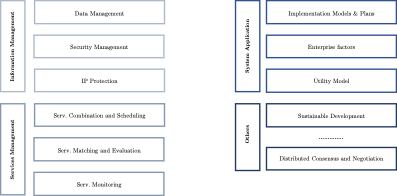
\includegraphics[height=6cm, keepaspectratio]{images/future-research-directions}
    \caption{Future research directions}
    \label{fig:future-research-directions}
\end{figure}

